\documentclass{article}
\usepackage[utf8x]{inputenc}
\usepackage{ucs}
\usepackage{amsmath} 
\usepackage{amsfonts}
\usepackage{marvosym}
\usepackage{wasysym}
\usepackage{upgreek}
\usepackage[english,russian]{babel}
\usepackage{graphicx}
\usepackage{float}
\usepackage{textcomp}
\usepackage{hyperref}
\usepackage{geometry}
  \geometry{left=2cm}
  \geometry{right=1.5cm}
  \geometry{top=1cm}
  \geometry{bottom=2cm}
\usepackage{tikz}
\usepackage{ccaption}
\usepackage{multicol}

\hypersetup{
   colorlinks=true,
   citecolor=blue,
   linkcolor=black,
   urlcolor=blue
}

\usepackage{listings}
%\setlength{\columnsep}{1.5cm}
%\setlength{\columnseprule}{0.2pt}

\usepackage[absolute]{textpos}

\usepackage{colortbl,graphicx,tikz}
\definecolor{X}{rgb}{.5,.5,.5}

\renewcommand{\thesubsection}{\arabic{subsection}}

\begin{document}
\pagenumbering{gobble}
\lstset{
  language=C,                % choose the language of the code
  basicstyle=\linespread{1.1}\ttfamily,
  columns=fixed,
  fontadjust=true,
  basewidth=0.5em,
  keywordstyle=\color{blue}\bfseries,
  commentstyle=\color{gray},
  stringstyle=\ttfamily\color{orange!50!black},
  showstringspaces=false,
  numbersep=5pt,
  numberstyle=\tiny\color{black},
  numberfirstline=true,
  stepnumber=1,                   % the step between two line-numbers.        
  numbersep=10pt,                  % how far the line-numbers are from the code
  backgroundcolor=\color{white},  % choose the background color. You must add \usepackage{color}
  showstringspaces=false,         % underline spaces within strings
  captionpos=b,                   % sets the caption-position to bottom
  breaklines=true,                % sets automatic line breaking
  breakatwhitespace=true,         % sets if automatic breaks should only happen at whitespace
  xleftmargin=.2in,
  extendedchars=\true,
  keepspaces = true,
}
\lstset{literate=%
   *{0}{{{\color{red!20!violet}0}}}1
    {1}{{{\color{red!20!violet}1}}}1
    {2}{{{\color{red!20!violet}2}}}1
    {3}{{{\color{red!20!violet}3}}}1
    {4}{{{\color{red!20!violet}4}}}1
    {5}{{{\color{red!20!violet}5}}}1
    {6}{{{\color{red!20!violet}6}}}1
    {7}{{{\color{red!20!violet}7}}}1
    {8}{{{\color{red!20!violet}8}}}1
    {9}{{{\color{red!20!violet}9}}}1
}


\title{Семинар \#4: Строки. Классные задачи.\vspace{-5ex}}\date{}\maketitle
\section*{\centering{Таблица ASCII}}
\begin{center}
\scalebox{1}{ 
\begin{tabular}{cc | cc | cc | cc | cc | cc | cc | cc | cc | cc} 
\rowcolor[rgb]{0,0.173,0.3255}
\textcolor{white}{Символ}&\textcolor{white}{Код}&
\textcolor{white}{С}&\textcolor{white}{К}&
\textcolor{white}{С}&\textcolor{white}{К}&
\textcolor{white}{С}&\textcolor{white}{К}&
\textcolor{white}{С}&\textcolor{white}{К}&
\textcolor{white}{С}&\textcolor{white}{К}&
\textcolor{white}{С}&\textcolor{white}{К}&
\textcolor{white}{С}&\textcolor{white}{К}&
\textcolor{white}{С}&\textcolor{white}{К}&
\textcolor{white}{С}&\textcolor{white}{К}
\\ 
\rowcolor[rgb]{0.89451,0.93588,0.97078} 
$\backslash$0 & 0  & \& & 38 & 0  & 48 & : & 58 & D & 68 & N & 78 & X & 88                & b & 98 & l & 108 & v & 118 \\
$\backslash$t & 9  & ' & 39 & 1   & 49 & ; & 59 & E & 69 & O & 79 & Y & 89                & c & 99 & m & 109 & w & 119 \\
\rowcolor[rgb]{0.89451,0.93588,0.97078} 
$\backslash$n & 10 & ( & 40 & 2   & 50 & < & 60 & F & 70 & P & 80 & Z & 90                & d & 100 & n & 110 & x & 120 \\
              &    & ) & 41 & 3   & 51 & = & 61 & G & 71 & Q & 81 & [ & 91                & e & 101 & o & 111 & y & 121 \\
              \rowcolor[rgb]{0.89451,0.93588,0.97078} 
(пробел)       & 32 & * & 42 & 4   & 52 & > & 62 & H & 72 & R & 82 & $\backslash$ & 92     & f & 102 & p & 112 & z & 122 \\
!             & 33 & + & 43 & 5   & 53 & ? & 63 & I & 73 & S & 83 & ] & 93                & g & 103 & q & 113 & \{ & 123 \\
\rowcolor[rgb]{0.89451,0.93588,0.97078} 
"             & 34 & , & 44 & 6   & 54 & @ & 64 & J & 74 & T & 84 & \textasciicircum & 94 & h & 104 & r & 114 & | & 124 \\
\#            & 35 & - & 45 & 7   & 55 & A & 65 & K & 75 & U & 85 & \_ & 95               & i & 105 & s & 115 & \} & 125 \\
\rowcolor[rgb]{0.89451,0.93588,0.97078} 
\$            & 36 & . & 46 & 8   & 56 & B & 66 & L & 76 & V & 86 & ` & 96                & j & 106 & t & 116 & \textasciitilde & 126 \\
\%            & 37 & / & 47 & 9   & 57 & C & 67 & M & 77 & W & 87 & a & 97                & k & 107 & u & 117 &  &  \\
 \end{tabular}
}
\end{center}

\section*{Часть 1: Символы.}
\subsection*{Тип \texttt{char} -- однобайтовое целое число}
Тип \texttt{char} -- это тип целочисленных чисел размером 1 байт (соответственно диапазон от \texttt{-128} до \texttt{127}).\\
Для считывания и печати переменных типа \texttt{char} используется спецификатор \texttt{\%hhi} (смотрите второй семинар).
\begin{lstlisting}
#include <stdio.h>
int main() {
    char a = 64;
    char b;
    scanf("%hhi", &b);
    printf("%hhi\n", a + b);
}
\end{lstlisting}
\begin{itemize}
\item Что напечатает эта программа, если на вход передать число \texttt{10}?
\item Что напечатает эта программа, если на вход передать число \texttt{100}?
\item Напишите программу, которая принимает на вход 2 числа, сохраняет их в переменных типа \texttt{char} и печатает результат произведения этих чисел.
\end{itemize}

\subsection*{Спецификатор \texttt{\%c} в функции \texttt{printf}}
\texttt{char} используется для хранения кодов символов. Функция \texttt{printf} со спецификатором \texttt{\%c} принимает на вход число и печатает соответствующий символ по таблице \texttt{ASCII}. Что напечатает следующая программа?
\begin{lstlisting}
#include <stdio.h>
int main() {
    printf("%c\n", 64);
}
\end{lstlisting}
\begin{itemize}
\item Напишите программу которая будет печатать символ \texttt{\^}
\item Вывести на экран все символы таблицы ASCII с номерами от 32 до 126 в следующем формате: 
\begin{lstlisting}
Symbol = A, Code = 65
\end{lstlisting}
\end{itemize}


\subsection*{Спецификатор \texttt{\%c} в функции \texttt{scanf}}
Функция \texttt{scanf} со спецификатором \texttt{\%c} считывает 1 символ и записывает код \texttt{ASCII} этого символа по соответствующему адресу.
\begin{lstlisting}
#include <stdio.h>
int main() {
    char x; 
    scanf("%c", &x);
    printf("%hhi\n", x);
}
\end{lstlisting}

\begin{itemize}
\item Измените программу выше так, чтобы она считывала 1 символ и печатала и этот символ и его код.
\item Напишите программу, которая будет постоянно считывать символы в цикле \texttt{while} и печатать эти символы и их коды. Программа должна заканчиваться после ввода с клавиатуры символа \texttt{q}.
\item Напишите программу, которая будет считывать символ и печатать:
\begin{itemize}
\item \texttt{Uppercase Letter}, если этот символ -- заглавная буква.
\item \texttt{Lowercase Letter}, если этот символ -- строчная буква.
\item \texttt{Digit}, если этот символ -- цифра.
\item \texttt{Other}, если это какой-то другой символ.
\end{itemize}
\end{itemize}

\subsection*{Символьные константы}
Для удобства работы с символами с языке были введены символьные константы. В коде они выглядят как символы в одинарных кавычках, но являются просто числами, соответствующими коду символа.
\begin{lstlisting}
#include <stdio.h>
int main() {
    int a = '@'; // Теперь a равно 64
    int b = '5'; // Теперь b равно 53
    printf("%d %d\n", a, b);
	
    // Проверьте себя. Что напечатает следующий код?
    printf("%d\n", '>');
    printf("%d\n", '1');
    printf("%d\n", 'a' + '0');
    printf("%d\n", '4' * '2');
    printf("%d\n", '7' - '0');
    printf("%c\n", 't' - 32);
    printf("%c\n", 'Z' + 'a' - 'A');
}
\end{lstlisting}

\begin{itemize}
\item Напишите программу, которая будет считывать символ и, если этот символ является строчной буквой, то делать эту букву заглавной и печатать её. Если символ -- не строчная буква, то нужно просто напечатать его.
\begin{center}
\begin{tabular}{ c | c }
 вход & выход \\ \hline
 \texttt{a} & \texttt{A}  \\ 
 \texttt{l} & \texttt{L}  \\ 
 \texttt{5} & \texttt{5}  \\ 
\end{tabular}
\end{center}
\end{itemize}
\newpage
\section*{Часть 2: Строки:}
Строки - это массивы чисел типа \texttt{char}, которые хранят коды символов. Самое значительное отличие строк от массивов это то, что конец строки задаётся как элемент массива символом с кодом \texttt{0}. 

\begin{center}
\includegraphics[scale=0.75]{../images/string_in_memory.png}
\end{center}

\subsection*{Объявление, инициализация и изменение строк}
Создавать строки можно также как и массивы, а можно и с помощью строки в двойных кавычках.
\begin{lstlisting}
int main() {
    char a[10] = {77, 73, 80, 84, 0};
    char b[10] = {'M', 'I', 'P', 'T', '\0'};
    char c[10] = "MIPT"; // Символ 0 поставится автоматически
	
    // Использовать = со строками можно только при создании, то есть это работать не будет:
    a = "FAKT";
    
    // Изменение элементов строк работает также как и у массивов
    a[1] = 'A';
}
\end{lstlisting}

\subsection*{Печать строк. Спецификатор \texttt{\%s}}
Обычные массивы нельзя печатать одной командой \texttt{printf}, но специально для строк ввели модификатор \texttt{\%s}, благодаря которому можно печатать и считывать строки одной командой.
\begin{lstlisting}
#include <stdio.h>
int main() {
    char a[10] = "MIPT";
    // Печатаем каждый символ по отдельности ( идём циклом до нулевого символа )
    for (int i = 0; a[i] != 0; ++i) {
        printf("%c", a[i]);
    }
    printf("\n");
	
    // Печатаем всю строку целиком
    printf("%s\n", a);
}
\end{lstlisting}

\begin{itemize}
\item Создайте строку \texttt{str} с содержимым \texttt{"Cat"} 3-мя разными способами и напечатайте её.
\item Измените созданную строку из прошлой задачи на \texttt{"Dog"} и снова напечатайте её.
\end{itemize}

\newpage
\subsection*{Считывание строк}
\begin{lstlisting}
#include <stdio.h>
int main() {
    char a[100];
    // Считываем каждый символ по отдельности до пробела или переноса строки ( сложный способ )
    for (int i = 0; 1; ++i) {
        char x;
        scanf("%c", &x);
        if (x == ' ' || x == '\n') {
            a[i] = 0;
            break;
        }
        a[i] = x;
    }
    printf("%s\n", a);
    
    // То же самое с помощью спецификатора %s ( простой способ )
    scanf("%s", a);
    printf("%s\n", a);
}
\end{lstlisting}

\begin{itemize}
\item Считайте число \texttt{n} и строку \texttt{str} и напечатайте её \texttt{n} раз через пробел. Для считывания используйте \texttt{scanf} со спецификатором \texttt{\%s}.
\item \textbf{Удвоение:} Считайте строку и напечатайте её удвоив каждый символ. Для итерации используйте тот факт, что в конце строки всегда должен стоять нулевой символ (символ с кодом \texttt{0}).
\begin{center}
\begin{tabular}{ c | c }
 вход & выход \\ \hline
 \texttt{Hello} & \texttt{HHeelllloo}  \\ 
 \texttt{MIPT} & \texttt{MMIIPPTT}  \\ 
\end{tabular}
\end{center}

\item \textbf{Усечение строки:} На вход подаётся строка. Усечь строку до первого символа точка \texttt{``.''}. Можно использовать только один вызов функции \texttt{printf}.
\begin{center}
\begin{tabular}{ c | c }
 вход & выход \\ \hline
 \texttt{judge.mipt.ru} & \texttt{judge} \\
 \texttt{A.B.C.} & \texttt{A}  \\ 
 \texttt{.com}   &   \\ 
\end{tabular}
\end{center}

\item \textbf{Сумма цифр:} На вход передаётся целое положительное число $n < 10^{10000}$. Нужно сумму цифр этого числа.
\textit{Подсказка:} Считайте это число как строку.
\begin{center}
\begin{tabular}{ c | c }
 вход & выход \\ \hline
  \texttt{97} & \texttt{16} \\
  \texttt{1234567890987654321234567890987654321} & \texttt{179} \\
\end{tabular}
\end{center}

\end{itemize}

\newpage
\subsection*{Строки и функции}
Строки передаются в функции также как и массивы. То есть при изменении строки внутри функции она меняется и снаружи. Но только при передаче строки не обязательно передавать её размер, так как граница строки задаётся нулевым символом. Пример функции, которая заменяет один символ в строке на другой:
\begin{lstlisting}
#include <stdio.h>
void change_letter(char str[], char from, char to) {
    int i = 0;
    while (str[i]) {
        if (str[i] == from) {
            str[i] = to;
        }
        i++;
    }
}
int main() {
    char a[100] = "Sapere aude";
    printf("%s\n", a);
    change_letter(a, 'e', '#');
    printf("%s\n", a);
}

\end{lstlisting}

\begin{itemize}
\item \textbf{Длина строки:} Напишите функцию \texttt{int get\_length(char str[])}, которая будет возвращать длину строки. Стандартную функцию \texttt{strlen} в этой задаче использовать нельзя. Проверьте эту функцию в \texttt{main()}.

\item \textbf{Переворот:} Напишите функцию \texttt{void reverse\_string(char str[])}, которая будет переворачивать строку строку. Проверьте эту функцию в \texttt{main()}.
\begin{center}
\begin{tabular}{ c | c }
 вход & выход \\ \hline
 \texttt{Hello!} & \texttt{!olleH}  \\ 
 \texttt{live} & \texttt{evil}  \\ 
 \texttt{Madam} & \texttt{madaM}  \\ 
\end{tabular}
\end{center}

\item \textbf{Uppercase:} Напишите функцию \texttt{void to\_upper\_case(char str[])}, которая будет переводить строку в верхний регистр. Проверьте эту функцию в \texttt{main()}.
\begin{center}
\begin{tabular}{ c | c }
 вход & выход \\ \hline
 \texttt{mipt} & \texttt{MIPT} \\
 \texttt{Hello!} & \texttt{HELLO!}  \\ 
 \texttt{Area51} & \texttt{AREA51} \\
\end{tabular}
\end{center}


\item \textbf{Шифр Цезаря:} Шифр Цезаря — это вид шифра подстановки, в котором каждый символ заменяется символом, находящимся на некотором постоянном числе позиций левее или правее него в алфавите. 
\begin{center}
\includegraphics[width=0.4\textwidth]{caesar.png}
\end{center}
Напишите функцию \texttt{void encrypt(char str[], int k)}, которая будет зашифровывать фразу шифром Цезаря.
\begin{center}
\begin{tabular}{ c | c }
 вход & выход \\ \hline
 \texttt{1 ABCZ} & \texttt{BCDA}\\
 \texttt{15 ZzZzZ} & \texttt{OoOoO} \\
 \texttt{7 The Fox Jumps Over The Dog} & \texttt{Aol Mve Qbtwz Vcly Aol Kvn} \\
 \texttt{13  Green Terra} & \texttt{Terra Green}
\end{tabular}
\end{center}


\end{itemize}

\subsection*{Считывание до заданного символа}
Как вы могли заметить, использование \texttt{scanf} с модификатором \texttt{\%s} считывает до первого пробельного символа. Чтобы считать всю строку (то есть до символа '\textbackslash n'), следует использовать модификатор \verb|%[^\n]|. \\
Пример программы, которая считывает строку и меняет пробелы на переносы строк:
\begin{lstlisting}
#include <stdio.h>
int main() {
    char str[100];
    scanf("%[^\n]", str);
    for (int i = 0; str[i]; i++){
        if (str[i] == ' ') {
            str[i] = '\n';
        }
    }
    printf("%s\n", str);
}
\end{lstlisting}

\begin{itemize}
\item \textbf{Переворот слов:} Используйте решение задачи \textbf{Переворот}, чтобы перевернуть каждое слово в строке.
\begin{center}
\begin{tabular}{ c | c }
 вход & выход \\ \hline
 \texttt{The Fox Jumps Over The Dog} & \texttt{ehT xoF spmuJ revO ehT goD} \\
\end{tabular}
\end{center}

\item \textbf{Сортировка символов:} Отсортируйте символы строки по их коду ASCII.
\begin{center}
\begin{tabular}{ c | c }
 вход & выход \\ \hline
 \texttt{MIPT} & \texttt{IMPT} \\
 \texttt{Majestic12} & \texttt{12Maceijst} \\
 \texttt{The Fox Jumps Over The Dog} & \quad \quad \quad \texttt{DFJOTTeeeghhmooprsuvx} \\
\end{tabular}
\end{center}

\item \textbf{Умножение на 3:} На вход передаётся целое положительное число $n < 10^{10000}$. Нужно напечатать это число, умноженное на 3.
\begin{center}
\begin{tabular}{ c | c }
 вход & выход \\ \hline
  \texttt{1234567890987654321234567890987654321} & \texttt{3703703672962962963703703672962962963} \\
\end{tabular}
\end{center}


\end{itemize}


\newpage
\section*{Часть 3: Стандартные функции библиотеки \texttt{string.h}:}
\begin{itemize}
\item \texttt{unsigned int strlen(char str[])} - возвращает длину строки
\item \texttt{char* strcpy (char a[], char b[]))} - копирует строку \texttt{b} в строку \texttt{a}, т.е. аналог \texttt{a = b}. Возвращает указатель на \texttt{a}.
\item \texttt{int strcmp(const char a[], char b[])} - лексикографическое сравнение строк (возвращает \texttt{0}, если строки одинаковые, положительное, если первая строка больше, и отрицательное, если меньше)
\item \texttt{char* strcat(char a[], char b[])} - приклеивает копию строки \texttt{b} к строке \texttt{a}, т.е. аналог \texttt{a += b}.
\item \texttt{char* strstr(char a[], char b[])} - ищет строку \texttt{b} в строке \texttt{a}. Возвращает указатель на первый символ вхождения строки \texttt{b} или \texttt{0} если такой строки нет.
\end{itemize}
\begin{lstlisting}
#include <stdio.h>
#include <string.h>
int main() {
	char a[100] = "Dog";
	char b[100] = "Mice";
	
	// Строки это массивы, поэтому их нельзя просто присваивать 
	a = "Cat"; // Это не будет работать! Нужно использовать strcpy:
	strcpy(a, "Cat");
	
	// Строки это массивы, поэтому их нельзя просто сравнивать
	a == b; // Это не будет работать! Нужно использовать strcmp:
	printf("%d\n", strcmp(a, b)); 
	
	// Конкатенация ( склейка ) строк. Можно воспринимать как +=
	strcat(a, b);
	printf("%s\n", a);
}
\end{lstlisting}

\begin{itemize}
\item Считайте строку и напечатайте её длину. Используйте функцию \texttt{strlen}.
\item \textbf{Обмен строк:} Напишите функцию \texttt{void swap\_strings(char a[], char b[])}, которая будет обменивать значениями две строки. Используйте стандартную функцию \texttt{strcpy}. Предполагается, что размер каждой из строк ограничен 100 символами.
\item \textbf{Поиск подстроки:} Считать 2 строки и проверить является ли вторая строка подстрокой первой строки. Вывести на экран \texttt{YES} или \texttt{NO} соответственно.
\end{itemize}

\subsection*{Чтение из файла}
Пример программу, которая подсчитывает количество слов в файле.
\begin{lstlisting}
#include <stdio.h>
#include <string.h>
int main() {
	// Считывание слов из файла
	FILE* infile = fopen("words.txt", "r");
	char words[500][100];
	int number_of_words = 0;
	while (fscanf(infile, "%s", words[number_of_words]) != -1) {
		number_of_words++;
	}
	fclose(infile);
}
\end{lstlisting}
\begin{itemize}
\item \textbf{Чтение из файла:} Напишите программу, которая будет считывать слова из файла и записывать их в массив \texttt{char words[1000][100]}. Когда в файле слов для считывания не останется, функция \texttt{fscanf} будет возвращать \texttt{-1}. После этого все слова должны быть напечатаны на экран через пробел. 
\item \textbf{Сортировка слов:} Напишите программу, которая будет считывать слова из файла и записывать их в массив \texttt{words}. После этого все слова должны быть отсортированы по алфавиту и записаны в файл \texttt{sorted\_words.txt}.
\end{itemize}

\end{document}